%!TEX root = ../these.tex

\section{Экстремальные свойства получаемого решения}
\label{sec:ccp.proof}

С практической точки зрения,
вышеописанный алгоритм оказывается
вполне работоспособным
и даёт хорошие результаты,
как в смысле времени работы,
так и качества получаемых решений.
Однако,
это чисто эмпирический результат,
так что было бы интересно получить
теоретические оценки качества работы
данного алгоритма.

На рис. \ref{fig:ccp-counter-example}
показан пример маршрута резки,
который не являясь кратчайшим,
тем не менее неё
может быть приведён к таковому
никакими индивидуальными сдвигами
точек врезки.
Таким образом, возникает вопрос,
при каких условиях предлагаемый алгоритм
гарантирует получение действительно
оптимального маршрута,
то есть другими словами,
глобального минимума оптимизационной задачи.

\begin{figure}[b]
  \begin{center}
  \begin{tikzpicture}[scale=2.7]
    \draw
      (1,-0.2) node(M3){} circle(0.027) node[below] {$M_3$}
      (-1,-0.2) node(M0){} circle(0.027) node[below] {$M_0$};
    \draw [thick,pattern=north west lines]
      (1.3,0) -- (2,0) -- (2,1) node[midway,left]{$C_2$} -- (1,1) node(M2x){} --
      (1, 1.1) -- (2.1,1.1) -- (2.1,-0.1) -- (1.3, -0.1) node(M2) {} --cycle
    % \draw [thick,pattern=north west lines]
      (-1.3,0) -- (-2,0) -- (-2,1) node[midway,right]{$C_1$} -- (-1,1) node(M1x){} --
      (-1, 1.1) -- (-2.1,1.1) -- (-2.1,-0.1) -- (-1.3, -0.1) node(M1){} --cycle;
    \draw[dashed]
      (M0) -- (M1) -- (M2) node[midway,above]{Глобальный минимум} -- (M3);
    \draw[dashed]
      (M0) -- (M1x) -- (M2x) node[midway,below]{Локальный минимум} -- (M3);
  \end{tikzpicture}
  \end{center}
  \caption{Два маршрута резки, доставляющие локальный и глобальный минимум}
  \label{fig:ccp-counter-example}
\end{figure}

Наиболее важным и одновременно
наиболее сложным является,
конечно, третий этап --
дискретная оптимизация
(фактически решение задачи коммивояжёра),
как с теоретической,
так и с практической точки зрения.
В данной же работе исследуется
второй шаг алгоритма --
непрерывная оптимизация.
Оказывается возможным сформулировать
некоторые утверждения относительно
получаемых в её ходе решений.

Итак,
рассмотрим следующую задачу:
пусть контуры
$C_i$
на плоскости состоят
только из отрезков прямых линий,
они не пересекаются и не вложены друг в друга.
Порядок обхода контуров
заранее задан.
Требуется найти кратчайшую ломаную линию,
чьи вершины лежат на заданных контурах
(в указанном порядке).

Мы начинаем с
(произвольной)
ломаной линии
$L_1$.
Далее для каждого контура
$C_i$
мы повторяем следующую операцию:
сдвигаем вершину ломаной
$M_i \in C_i$
в такое положение,
которое минимизирует полную
длину ломаной,
при этом остальные вершины
$M_j$
($j \ne i$)
неподвижны.
Это сводится к несложной геометрической
задаче нахождения точки,
для которой сумма расстояний
до двух других фиксированных точек
минимальна.

В процессе таких пошаговых сдвигов
мы получаем последовательность
ломаных линий
$\{L_k\}$,
причём последовательность
длин этих ломаных линий
по построению монотонно убывает.
Обозначим
$m = \inf |L_k|$
(точная нижняя граница длин ломаных линий)
и пусть
$L_*$  --
ломаная линия длины
$m$,
то есть предельная точка
последовательности ломаных линий
$\{L_k\}$.
В качестве метрики на пространстве ломаных линий
можно использовать сумму расстояний между
вершинами с одинаковыми номерами.

В реальных примерах
стабилизация последовательности ломаных
происходит буквально в течение
нескольких итераций
(не более 10)
и ломаная
$L_*$
действительно получается
во всех численных экспериментах

По построению,
длина ломаной
$L_*$
не может быть уменьшена никаким сдвигом
одной из её вершин
(в рамках содержащего её контура),
также как и сдвигом
любого количества её вершин,
не являющихся соседними.

\subsection{Локальный минимум}

\begin{proposition}
  Сдвиг нескольких соседних вершин ломаной
  $L_*$
  таким образом,
  что сдвигаемые вершины остаются на тех же самых сегментах
  контуров,
  не приводит к уменьшению полной длины ломаной.
\end{proposition}

\begin{proof}
Рассмотрим сдвиг
\textit{двух}
соседних вершин.
Обозначим четыре последовательных вершины ломаной
$L_*$
за
$M_{i-1}, M_i, M_{i+1}, M_{i+2}$.

Пусть точки
$M_i \in S_i,
M_{i+1} \in S_{i+1}$
лежат на прямолинейных сегментах
соответствующих контуров
$S_i \subset C_i,
S_{i+1} \subset C_{i+1}$.

Докажем, что:
$$
\forall M'_i \in S_i,
M'_{i+1} \in S_{i+1}
:
|M_{i-1} M'_i M'_{i+1} M_{i+2}|
\geqslant
|M_{i-1} M_i M_{i+1} M_{i+2}|
$$

Для произвольной вершины
$M'_i \in S_i$:
$|M_{i-1} M'_i M_{i+1} M_{i+2}|$
минимально, когда
$M'_i=M_i$,
и аналогично
для произвольной вершины
$M'_{i+1} \in S_{i+1}$:
$|M_{i-1} M_i M'_{i+1} M_{i+2}|$
минимально, когда
$M'_{i+1}=M_{i+1}$.

Предположим, что
$$
\exists M'_i \in S_i,
\exists M'_{i+1} \in S_{i+1}
:
|M_{i-1} M'_i M'_{i+1} M_{i+2}|
<
|M_{i-1} M_i M_{i+1} M_{i+2}|
$$

Очевидно, что
$
M'_i \ne M_i,
M'_{i+1} \ne M_{i+1}
$.

Введём обозначение
$
M_i(s)=M_i+s \cdot \overrightarrow{M_i M'_i}
$,
$
  M_{i+1}(t)= M_{i+1}+t \cdot \overrightarrow{M_{i+1} M'_{i+1}}
$
($s,t \in[0,1]$),
$f(s,t)=
|M_{i-1} M_i(s) M_{i+1}(t) M_{i+2}|
$.

Но положения вершин
$M_i$ and $M_{i+1}$
выбраны так, что:
\begin{equation}
\label{eq:ccp-partials}
\frac{\partial f(s,t)}{\partial s} \Big|_{(0,0)} \geqslant 0,
\frac{\partial f(s,t)}{\partial t} \Big|_{(0,0)} \geqslant 0
\end{equation}

Если,
например,
$\partial f(s,t) / \partial s \big|_{(0,0)} = 0$,
то это может быть только если точки
$M_{i-1}, M_i, M_{i+1}$
лежат на одной прямой
(когда
$M_{i-1}$
и
$M_{i+1}$
по одну сторону от
$S_i$;
в противном случае
заменяем
$M_{i-1}$
на её отражение относительно
$S_i$).
Таким образом,
если одновременно
$$
\frac{\partial f(s,t)}{\partial s} \Big|_{(0,0)}
= 0 =
\frac{\partial f(s,t)}{\partial t} \Big|_{(0,0)}
$$
то значит все четыре точки
$M_{i-1}, M_i, M_{i+1}, M_{i+2}$
лежат на одной прямой
и проходящая через них ломаная
фактически является отрезком прямой
и заведомо кратчайшая,
не может быть сделана короче.

Рассмотрим теперь случай,
когда хотя бы одна из производных в
\eqref{eq:ccp-partials}
не равна нулю.
Обозначим
$\varphi(t)=f(t,t)$.

$$
\frac{d\varphi}{dt} \Big|_0 =
\frac{\partial f(s,t)}{\partial s} \Big|_{(0,0)}
+
\frac{\partial f(s,t)}{\partial t} \Big|_{(0,0)}
>0
$$

Это значит, что
$\exists \tau^* \in [0,1]$:
$\varphi(\tau^*) > \varphi(0)$.
Но по нашему предположению
$\varphi(1)<\varphi(0)$,
то есть
$\varphi(0)<\varphi(\tau^*)>\varphi(1)$.

Теперь заметим, что
$\varphi(t)$
представляет собой сумму четырёх слагаемых вида
$\sqrt{(a+b\cdot t)^2 + (c+d \cdot t)^2}$,
и каждое из этих слагаемых имеет
положительную вторую производную,
так что и
$d^2\varphi(t)/dt^2 \geqslant 0$,
а значит функция
$\varphi(t)$
является выпуклой на
$[0,1]$
и не может принимать
во внутренней точке интервала
значения большие,
чем на его концах.

Значит,
наше предположение невозможно.

Мы рассмотрели сдвиг \textit{двух}
соседних вершин ломаной.
Для большего числа соседних вершин
доказательство аналогично,
только более громоздко.

Окончательно,
мы доказали, что ломаная линия
$L_*$
представляет собой
\textbf{локальный}
минимум.
\end{proof}

\subsection{Глобальный минимум}

Перейдём к \textit{достаточному}
условию того,
что ломаная
$L_*$
является глобальным минимумом.

Пусть
$M_i \in C_i$ --
вершина ломаной
$L_*$.
Соседние вершины
$M_{i-1}$
и
$M_{i+1}$
находятся вне
$C_i$,
поскольку по условию задачи
мы исключили вложенные контуры
По построению
$L_*$:
$\forall M'_i \in C_i:
|M_{i-1} M_i|+|M_i M_{i+1}|
\leqslant
|M_{i-1} M'_i|+|M'_i M_{i+1}|
$.

\begin{condition}
  \label{cond:ccp-or}
Пусть выполняется
\textbf{одно}
из следующих условий
(см.~рис.~\ref{fig:ccp-sufficient-two}):
\begin{enumerate}
  \item
  Сегмент
  $M_{i-1} M_{i+1}$
  пересекает контур
  $C_i$,
  то есть
  $M_i \in M_{i-1} M_{i+1}$,
  рис.~\ref{fig:ccp-thru}
  \item
  Касательная в точке
  $M_i$
  к эллипсу с фокусами
  $M_{i-1}$
  и
  $M_{i+1}$
  и проходящему через
  $M_i$,
  разделяет эллипс и контур
  $C_i$,
  рис.~\ref{fig:ccp-ellipse}
\end{enumerate}
\end{condition}

\begin{figure}
  \centering
  \subfloat[Маршрут пересекает контур]{
    \label{fig:ccp-thru}
    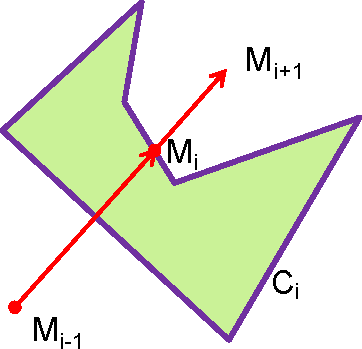
\includegraphics{proof/thru.pdf}
  }
  \subfloat[Касательная отделяет контур]{
    \label{fig:ccp-ellipse}
    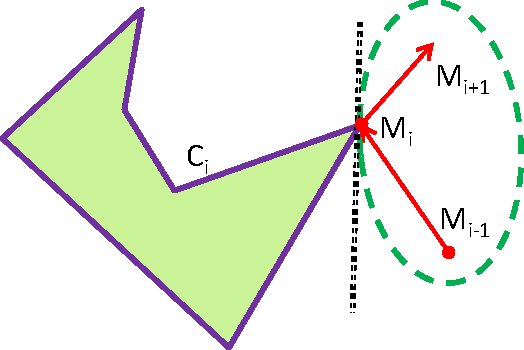
\includegraphics{proof/ellipse.pdf}
  }
  \caption{Достаточные условия глобального минимума}
  \label{fig:ccp-sufficient-two}
\end{figure}

\begin{proposition}
Если условие
\ref{cond:ccp-or}
выполняется для
(всех контуров)
$L_*$,
то
при сдвиге нескольких соседних вершин ломаной
$L_*$
в рамках содержащих их контуров,
полная длина ломаной не уменьшается,
то есть ломаная
$L_*$
представляет собой глобальный минимум.
\end{proposition}

\begin{proof}
Используя те же обозначения,
рассмотрим четыре соседних вершины
$M_{i-1}, M_i, M_{i+1}, M_{i+2} \in L_*$.
$M_i \in  C_i,
M_{i+1} \in C_{i+1}$.

Предположим, что
$$
\exists M'_i \in C_i,
\exists M'_{i+1} \in C_{i+1}:
|M_{i-1} M'_i M'_{i+1} M_{i+2}|
<
|M_{i-1} M_i M_{i+1} M_{i+2}|
$$

Снова,
$
M'_i \ne M_i,
M'_{i+1} \ne M_{i+1}
$.

Обозначим
$
M_i(s)=M_i+s \cdot \overrightarrow{M_i M'_i}
$,
$
  M_{i+1}(t)= M_{i+1}+t \cdot \overrightarrow{M_{i+1} M'_{i+1}}
$
($s,t \in[0,1]$),
$f(s,t)=
|M_{i-1} M_i(s) M_{i+1}(t) M_{i+2}|
$.

Но теперь условие
\ref{cond:ccp-or}
гарантирует, что
$f(s,0)\geqslant f(0,0)$
для
$s\in[0,1]$,
то есть снова
\begin{equation}
  \frac{\partial f(s,t)}{\partial s} \Big|_{(0,0)} \geqslant 0,
  \frac{\partial f(s,t)}{\partial t} \Big|_{(0,0)} \geqslant 0
  % \label{partials}
\end{equation}

Поэтому остальная часть предыдущего доказательства
повторяется отсюда без изменений.
\end{proof}

Предположим,
что кроме
$L_*$
существует другая ломаная,
также являющаяся глобальным минимумом.
Тогда из доказательства следует,
что они представляют собой одну и ту же
линию
(как множество точек)
и отличаются только положением вершин,
то есть тем, какие именно пересечения
с контурами
выбраны в качестве вершин ломаных линий.

Условие \ref{cond:ccp-or}
легко проверяется программно,
однако его можно ещё упростить с тем,
чтобы в большинстве практических случаев
его можно было проверить просто визуально,
буквально <<на глаз>>.

\begin{condition}
  \label{cond:ccp-four}
  Выполняется \textbf{любое} из условий
  (см.~рис.~\ref{fig:ccp-sufficient-weak}):
  \begin{enumerate}
    \item
    Сегмент
    $M_{i-1} M_{i+1}$
    пересекает контур
    $C_i$:
    $M_i \in M_{i-1} M_{i+1}$,
    рис.~\ref{fig:ccp-thru-again}
    \item
    Если вершина
    $M_i$
    является внутренней точкой одного из
    отрезков контура
    $C_i$
    и при этом весь контур расположен
    по одну сторону линии,
    проходящей через этот отрезок
    (это и есть касательная,
    которую использует условие~\ref{cond:ccp-or};
    иначе существовала бы лучшая вершина
    $M'_i\in C_i$),
    рис.~\ref{fig:ccp-edge}
    \item
    Если вершина
    $M_i$
    является также вершиной контура
    $C_i$
    (принадлежит сразу двум его отрезкам)
    и при этом весь контур находится
    внутри угла,
    образованного лучами,
    идущими из вершины
    $M_i$
    вдоль этих двух отрезков,
    рис.~\ref{fig:ccp-corner}
    \item
    Если контур
    $C_i$
    ограничивает собой выпуклый
    многоугольник
    $\widetilde C_i$,
    рис.~\ref{fig:ccp-convex}
  \end{enumerate}
\end{condition}

\begin{figure}
  \centering
  \subfloat[Маршрут пересекает контур]{
    \label{fig:ccp-thru-again}
    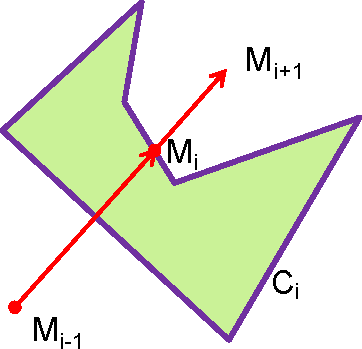
\includegraphics{proof/thru.pdf}
  }
  \subfloat[Точка врезки на ребре]{
    \label{fig:ccp-edge}
    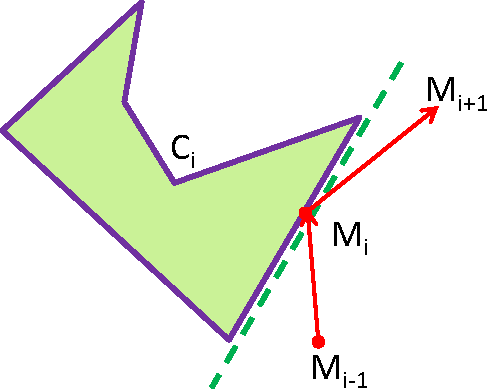
\includegraphics{proof/edge.pdf}
  }
  \\
  \subfloat[Врезка в вершину контура]{
    \label{fig:ccp-corner}
    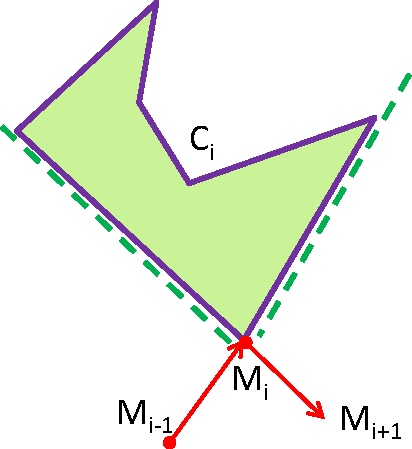
\includegraphics{proof/corner.pdf}
  }
  \subfloat[Выпуклый контур]{
    \label{fig:ccp-convex}
    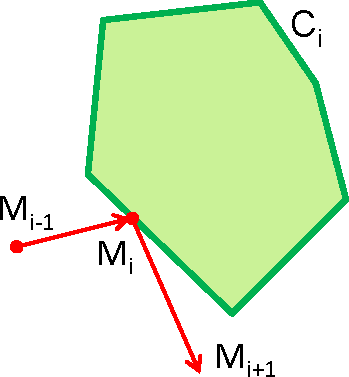
\includegraphics{proof/convex.pdf}
  }
  \caption{Ослабленное условие глобального минимума}
  \label{fig:ccp-sufficient-weak}
\end{figure}
